\documentclass[12pt]{article}
\usepackage{graphicx} % Required for inserting images
\usepackage{amsmath}
\usepackage{geometry}
\geometry{margin=1in}
\usepackage{amssymb}

\title{Population Econ HW3}
\author{YU HSIANG LIEN 1A202G34}
\date{December 2023}

\begin{document}

\maketitle

\section{Chapter 7}
\begin{enumerate}
    \item [\textbf{Q1}] 
    
    \begin{enumerate}
        \item[\textbf{(a)}] In the presence of an under ground economy, there is a possibillity that it 
        will result in a GINI coefficient that either over-state or under-state poverty 
        depand on the size and nature of the undeground economy.
        \newline

        I: If the undeground economy sontribute to the population that is in the low-income side,
        it will lead to a `over-state' of poverty. Since in reality these low-income population actually 
        have more income than the data indicate.
        \newline

        II: On the other hand, if the underground economy contribute to the population that is in the 
        high-income side, it will lead to a `under-state' of poverty. Since in reality, those high-income 
        population actually enjoying more income than the data indicate and thus there is a larger
        inequlity in reality.

        \item[\textbf{(b)}]
        Poorest $ 90\%\Rightarrow$ 10000 income 

        Rest $ 10\%\Rightarrow$ 110000 income 

        $\Rightarrow$ The income share of the poorest 90\% is: $\frac{9 \times 10000}{(9 \times 10000) + 110000}$ = $\frac{90000}{200000}$  = 0.45 

        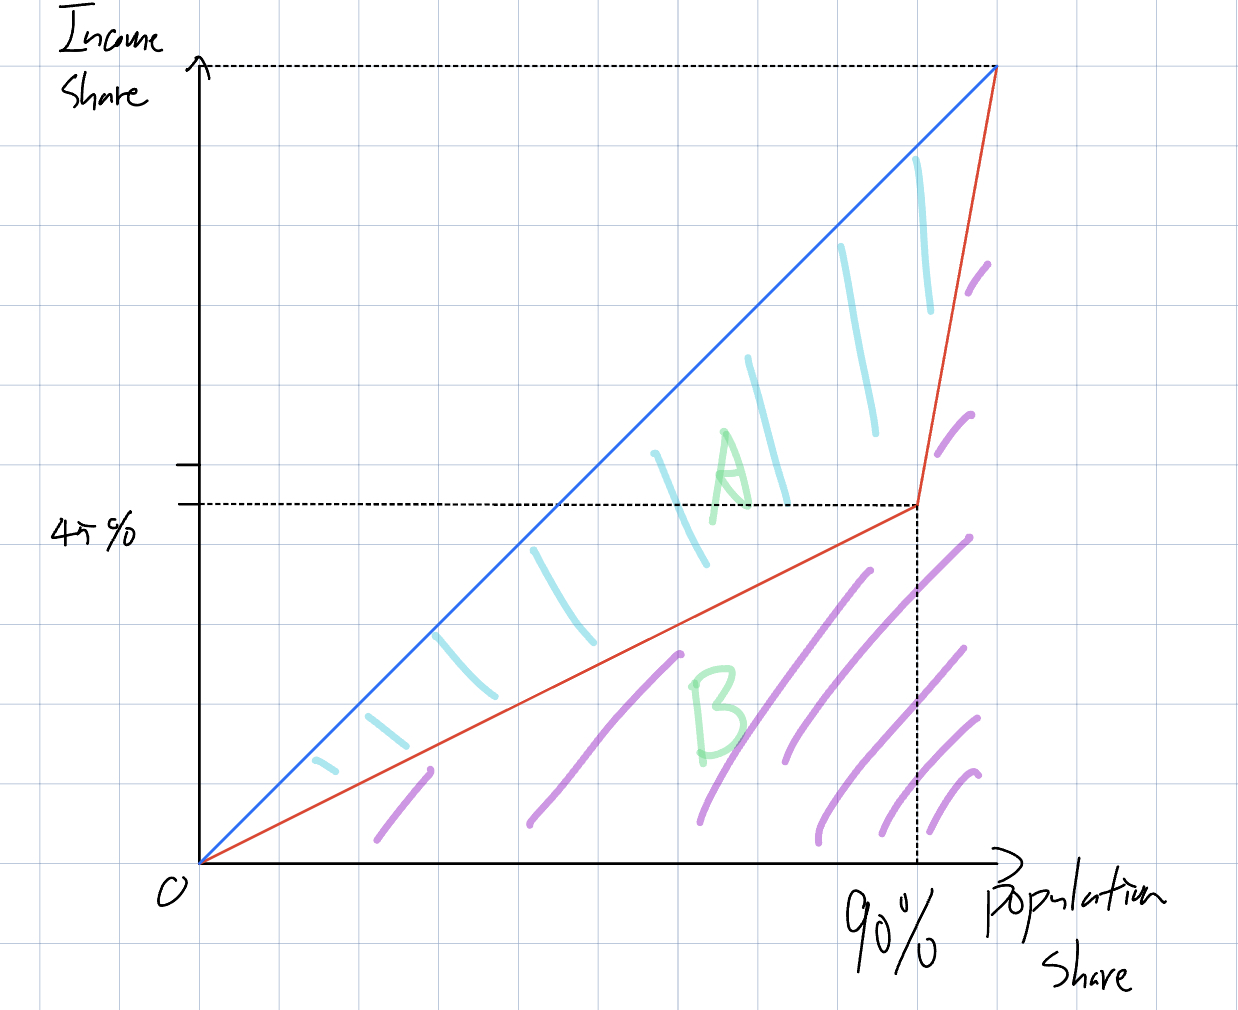
\includegraphics[width=0.5\linewidth]{hw3_img1.jpeg} \newpage

        Gini coefficient = $\frac{A}{A + B}$

        $\Rightarrow \frac{\frac{100}{2} - (\frac{9 \times 4.5}{2} + \frac{4.5 + 10}{2})}{\frac{10 \times 10}{2}} = \frac{50 - (20.25 + 7.25)}{50} = 0.45$ 

        \textbf{Ans}: Gini coefficient = 0.45


        \item[\textbf{(c)}]  
        Poorest $ 90\%\Rightarrow$ 15000 income 

        Rest $ 10\%\Rightarrow$ 110000 income 

        $\Rightarrow$ The income share of the poorest 90\% is: $\frac{9 \times 15000}{(9 \times 15000) + 110000}$ = $\frac{135000}{245000} = \frac{27}{49}$   

        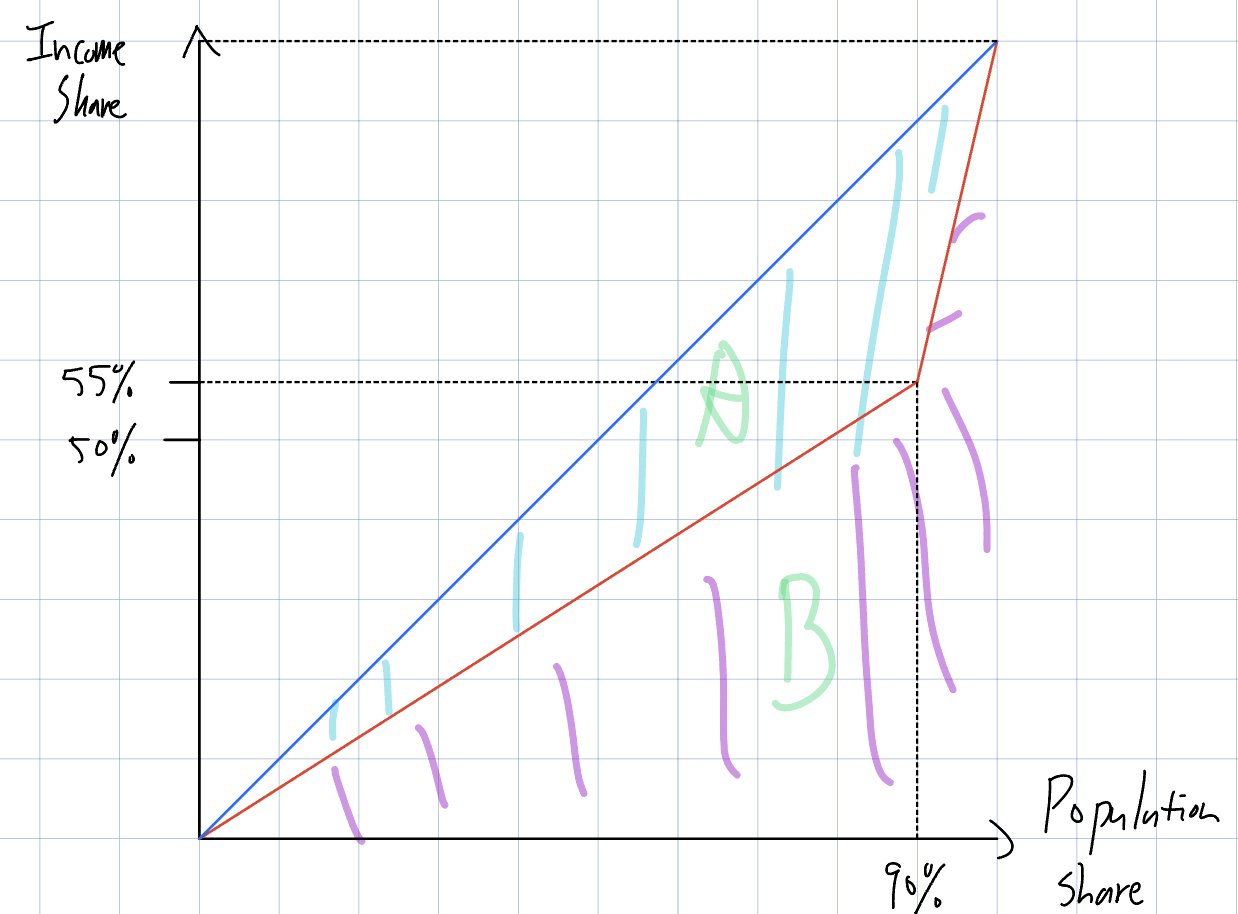
\includegraphics[width=0.5\linewidth]{hw3_img2.jpeg} 

        Gini coefficient = $\frac{A}{A + B}$ 

        $\Rightarrow \frac{\frac{100}{2} - (\frac{9 \times 5.5}{2} + \frac{5.5 + 10}{2})}{\frac{10 \times 10}{2}} = \frac{50 - (24.75 + 7.75)}{50} = \frac{50 - 32.5}{50} = \frac{17.5}{50} = 0.35$

        \textbf{Ans}: Gini coefficient = 0.35
    \end{enumerate}
    
    
    \item [\textbf{Q2}]
    Bottom 50 \% $\Rightarrow$ P \% of nation income
    Upper 50 \% $\Rightarrow$ (1-P) \% of nation income
    
    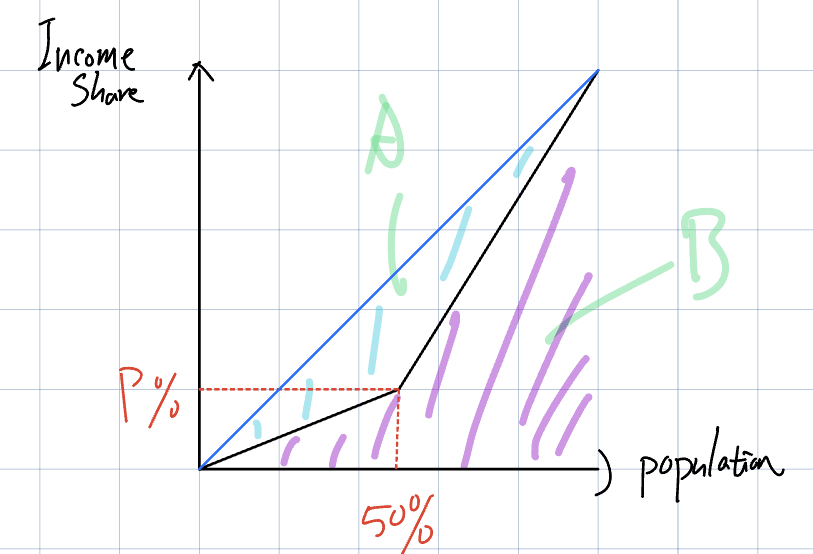
\includegraphics[width=0.5\linewidth]{hw3_img3.jpeg}
    
    \begin{enumerate}
        \item[\textbf{(a)}]
        Gini coefficient $\Rightarrow \frac{1}{2} - \frac{\frac{P}{100} \times 0.5}{2} - \frac{(\frac{P}{100} + 1) \times 0.5}{2} = 0.25 - \frac{P}{200} = 0.25 - 0.005P$
        
        $\Rightarrow \frac{0.25 - 0.005P}{0.2} = \frac{5 - 0.1P}{10} = 0.5- 0.01P$

        \textbf{Ans}: Gini coefficient = 0.5 - 0.01P

        \item[\textbf{(b)}] $90 - 10$ gap
        
        Top 10\% $\Rightarrow (1 - \frac{P}{100}) \times \frac{1}{5}$, \@ Bottom 10\% $\Rightarrow (\frac{P}{100}) \times \frac{1}{5}$

        $90 - 10 gap = \frac{1 - \frac{P}{100}}{5} - \frac{\frac{P}{100}}{5} = \frac{1 - \frac{2P}{100}}{5} = \frac{250 - P}{250}$ 
        
        \textbf{Ans}: $90 - 10$ gap: $\frac{250 - P}{250}$
    \end{enumerate}
    
    \item [\textbf{Q3}]
    
    \begin{enumerate}
        \item[\textbf{(a)}]
        The Market-determined rental rate to an efficiency unit falls: \newline
        $\Rightarrow$ This will made OJT less attractive since right now the benefit of OJT investment is lower, and thus
        decrease the investment on OJT.\@
        \item[\textbf{(b)}]
        Jill's discount rate increase: \newline
        $\Rightarrow$ When Jill's discount rate increase, it means that he is more impatient and the future
        benefit is less attractive in present. This will make OJT investment less attractive, as the future return from OJT 
        will be discount heavily and thus result in an decrease in OJT investment.
        \item[\textbf{(c)}]
        Government passes legislation delaying the retirement age util age 70: \newline
        $\Rightarrow$ This will likely to increase Jill's investment on OJT since right now the lifetime total work hour
        is longer, so the time that Jill can enjoy the benefit come from OJT is longer. And thus this will make OJT investment
        more attractive and result in an increase in OJT investment.
        \item[\textbf{(d)}]
        Technological progress is such that much of the OJT acquired at any given age becomes obsolete within the next 10 years: \newline
        $\Rightarrow$ This will result in a opposite outcome to the previous question. Right now due to the Technological advance, Jill have only 10 years, a much shorter time
        time that he can enjoy the benefit from OJT.\@ Thus the total benefit come from OJT is reduced heavily and make OJT investment less attractive, and finally lead to 
        a decrease in OJT investment.
    \end{enumerate}
    

\end{enumerate}

\section{Chapter 5}
\begin{enumerate}
    \item [\textbf{Q1}]
    
    $U = \sqrt{w} - 2x$, \@ Clean job $\Rightarrow x = 0$, \@ Dirty job $\Rightarrow x = 1$, \@ Clean job wage = 16

    $U_\text{Clean} = \sqrt{16} - 2 \times 0 = 4 - 0 = 4$

    $\Rightarrow$ The $U_\text{Dirty}$ have to be equal to $U_\text{Clean}$

    $\Rightarrow 4 = U_\text{Dirty} = \sqrt{w} - 2 \Rightarrow \sqrt{w} = 6 \Rightarrow w = 36$

    Compensating wage differential = 36 - 16 = 20

    \textbf{Ans}: Dirty job wage = 36, Compensating wage differential = 20



    \item [\textbf{Q2}]
    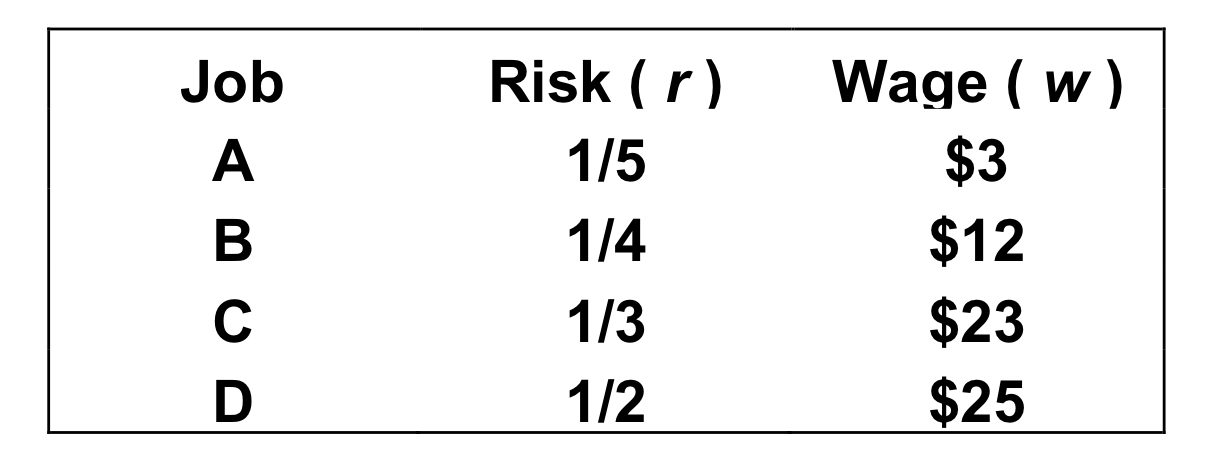
\includegraphics[width=0.5\linewidth]{hw3_img4.jpeg}

    $u(w, r) = w + \frac{1}{r^2}$

    (1)

    $\Rightarrow u_A = 3 + 25 = 28, u_B = 12 + 16 = 28,\\ u_C = 23 + 9 = 32, u_D = 25 + 4 = 29$

    $\Rightarrow$ Job C got the highest utility

    \textbf{Ans}: Worker choose to work at Job C

    (2)

    Risk factor must be $\frac{1}{5}$ 
    
    $\Rightarrow u_A\prime = w_A\prime + (\frac{1}{5})^2 = 32 \Rightarrow w_A\prime = 32 - 25 = 7$

    \textbf{Ans}: New job A wage after government regulation = 7

    \item [\textbf{Q3}]
    
    Total labor = 25000, Ashto: $W_A = 20 - 0.0024E_A$, Benton: $W_B = 20 - 0.0004E_B$

    \begin{enumerate}
        \item [I]: If $W_B - W_A = 0 \Rightarrow \frac{E_B}{E_B + E_A} = 0 \Rightarrow E_B = 0, E_A = 25000$\\
        $\Rightarrow W_A = 20 - 0.0024 \times 25000 = -40 \Rightarrow \textbf{Not Possible}$
        \item [II]: If $W_B - W_A = 1 \Rightarrow \frac{E_B}{E_B + E_A} = \frac{1}{5} \Rightarrow E_B = 5000, E_A = 20000$\\
        $\Rightarrow W_A = 20 - 0.0024 \times 20000 = -28 \Rightarrow \textbf{Not Possible}$
        \item [III]: If $W_B - W_A = 2 \Rightarrow \frac{E_B}{E_B + E_A} = \frac{2}{5} \Rightarrow E_B = 10000, E_A = 15000$\\
        $\Rightarrow W_A = 20 - 0.0024 \times 15000 = -16 \Rightarrow \textbf{Not Possible}$
        \item [IV]: If $W_B - W_A = 3 \Rightarrow \frac{E_B}{E_B + E_A} = \frac{3}{5} \Rightarrow E_B = 15000, E_A = 10000$\\
        $\Rightarrow W_A = 20 - 0.0024 \times 10000 = -4 \Rightarrow \textbf{Not Possible}$
        \item [V]: If $W_B - W_A = 4 \Rightarrow \frac{E_B}{E_B + E_A} = \frac{4}{5} \Rightarrow E_B = 20000, E_A = 5000$\\
        $\Rightarrow W_A = 20 - 0.0024 \times 5000 = 8 \Rightarrow W_B = 8 + 4 = 12$\\
        $\Rightarrow 12 = 20 - 0.0004E_B \Rightarrow E_B = 8 \div 0.0004 = 20000$\\
        $\Rightarrow$ \textbf{Market Equilibrium}
        \item [VI]: If $W_B - W_A = 5 \Rightarrow \frac{E_B}{E_B + E_A} = 1 \Rightarrow E_B = 250000, E_A = 0$\\
        $\Rightarrow W_A = 20 - 0.0024 \times 0 = 25 \Rightarrow W_B = 20 + 4 = 24$\\
        $\Rightarrow 24 = 0.0004E_B \Rightarrow E_B = 24 \div 0.0004 = 120000 \Rightarrow \textbf{Contradict}$\\

        \textbf{Ans}: $E_A = 5000, E_B = 20000, W_A = 8, W_B = 12, \text{Wage differential} = 4$
        
    \end{enumerate}

\end{enumerate}

\section{Chapter 8}
\begin{enumerate}
    \item [\textbf{Q1}]
    Discount Rate = 10\%, Pennsylvania income = 20000, Illinois income = 22000

    $\Rightarrow$ Pennsylvania lifetime income = $20000 + \frac{20000}{1.1} + \frac{20000}{1.1^2} = 20000 + 18181.82 + 16528.93 \\= 54710.75$

    $\Rightarrow$ Illinois lifetime income = $22000 + \frac{22000}{1.1} + \frac{22000}{1.1^2} = 22000 + 20000 + 18181.82\\ = 60181.82$

    $\Rightarrow$ Max cost of migration = $60181.82 - 54710.75 = 5471.07$

    \textbf{Ans}: Max cost = 5471.07
    \newpage

    \item [\textbf{Q2}]
    Moving Cost = 25000, 

    Patrick lifetime earning: Seattle = 125000, Atlanta = 155000

    Rachel lifetime earning: Seattle = 500000, Atlanta = 510000

    $\Rightarrow$ Net gain for Patrick if move = $155000 - 125000 = 30000 > 25000$

    $\Rightarrow$ Net gain for Rachel if move = $510000 - 500000 = 10000 < 25000$

    $\Rightarrow$ Patrcick is a \textbf{Tied-Mover} since his net gain is larger than cost,\\ Rachel is a \textbf{Tied-Stayer} since her net gain is smaller than moving cost.

    \item [\textbf{Q3}] Impact of remote work

    (1) \textbf{Increse Job  Mobility}

    $\Rightarrow$ Since with remote work, it enhance job mobility by reducing the geographical constraints on job seekers. 
    Workers may be more willing to consider job opportunities in different locations, which is formerly impossible to reach without moving, 
    as physical distance to the workplace becomes less crucial. And thus increase job mobility.

    (2) \textbf{Unclear impact on internal migration}

    \textbf{Possibiliy Decrease} \\$\Rightarrow$ Remote work could lead to a decrease in internal migration rates. 
    If employees can effectively work from anywhere, the traditional reasons for moving, such as job opportunities in a specific city, 
    might become less compelling. And thus decrease internal migration.

    \textbf{Possibiliy Increase} \\$\Rightarrow$ With the ability to remote work, 
    workers may choose to live in cities that align with their lifestyle preferences rather than solely for job opportunities. 
    This could lead to a redistribution of the population, with people opting for locations with lower costs of living or better quality of life.
    And thus increasing internal migration.

    \item [\textbf{Q4}] Roy Model of migration
    
    (1) This situation will happened if the host country can provide higher wage for 
    low-skill workers that is simply seeking for a higher wage, and also can provide better environment such as career opportunity and lifestyle and possibily higher wage for high-skill population. 
    If there is such a case, the scource country might experience both an outflow of low-skill workers and high-skill worker at the same time.\newpage

    (2)

    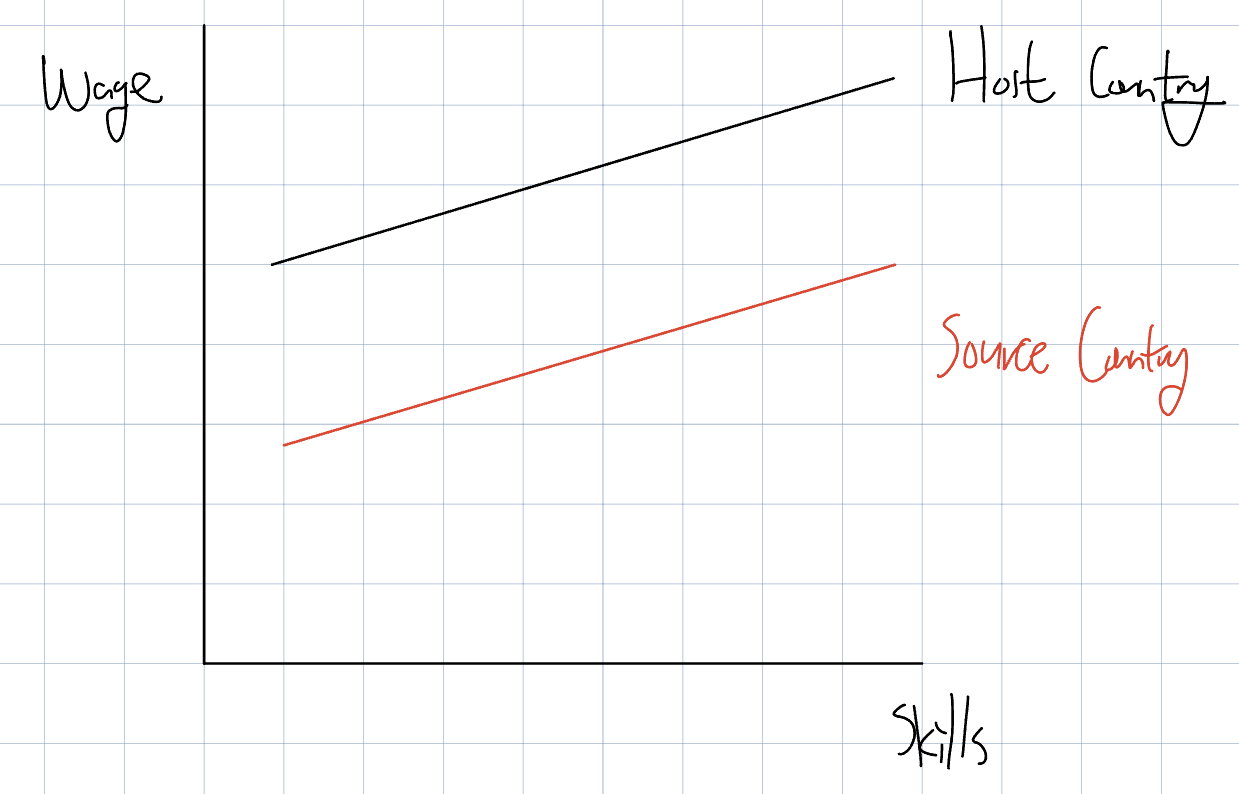
\includegraphics[width=1\linewidth]{hw3_img5.jpeg}


\end{enumerate}

\end{document}